\documentclass{snedecorbeamer}

%% Slide numbers
\usepackage{appendixnumberbeamer}

%% References
\usepackage{cleveref}

%% Figures
\usepackage{subcaption}

%% Captions
%%% Small font
\captionsetup{font=tiny}
%%% Remove caption
\setbeamertemplate{caption}{\raggedright\insertcaption\par}

%% Footnotes
%%% Small font https://tex.stackexchange.com/a/146021
\setbeamerfont{footnote}{size=\tiny}

%% Symbol resizing
\usepackage{scalerel}

%% Diagrams
%%% General tikz preamble
\usepackage{tikz}
\usetikzlibrary{positioning,decorations.pathreplacing,quotes,overlay-beamer-styles}

%% Create section slides
%%% https://tex.stackexchange.com/a/117661
\AtBeginSection{\frame{\sectionpage}}
\AtBeginSubsection{\frame{\subsectionpage}}

%%
\newcommand{\appendixlink}[1]{
  \hyperlink{#1}{\resizebox{!}{1.5ex}{\beamergotobutton{appendix}}}
}

%% Some math
  \newcommand{\calT}{\mathcal{T}}
  \newcommand{\dt}{\, \mathrm{d}t}
  \newcommand{\du}{\, \mathrm{d}u}
  \newcommand{\dv}{\, \mathrm{d}v}
  \newcommand{\w}{\omega}
  \newcommand{\dotsq}{{\left[d(t)\right]}^2}
  \newcommand{\fall}{\,~\forall~\,}

% Setup ------------------------------------------------------------------------
\graphicspath{{include/}}

\title{\textbf{Automatic Relevance Determination} \\
  for Gaussian Processes with Functional Inputs}

\renewcommand*{\thefootnote}{\fnsymbol{footnote}}
\author[Damiano et al]{
  \textbf{Luis Damiano}\footnote[2]{
    \tiny{\href{mailto:ldamiano@iastate.edu}{ldamiano@iastate.edu}}
  }}

\institute{
  Department of Statistics, Iowa State University
}

\date[April 7th, 2023]{
  \tiny{Department of Statistics \\
    Iowa State University} \\
  April 7th, 2023}

\begin{document}

% Title page -------------------------------------------------------------------
\begin{frame}
  \titlepage{}
  {
    \tiny{
      Funded, in part, by
      \begin{itemize}
      \item[-] ISU Presidential Interdisciplinary
	Research Initiative on C-CHANGE:~Science for a Changing
	Agriculture
      \item[-] Foundation for Food and Agriculture Research
	Grant ID: CA18-SS-0000000278
      \end{itemize}
    }
  }
\end{frame}

% Introduction -----------------------------------------------------------------
\begin{frame}
  \frametitle{Outline}
  \framesubtitle{Roadmap from a scientific problem to a statistical framework}

  \begingroup
  \setbeamersize{description width=-\labelsep}
%   \begin{description}
%   \item[Motivation] \mbox{}\\
%     Surrogates for computer models with functional inputs
%   \item[Automatic Dynamic Relevance Determination] \mbox{}\\
%     \href{https://doi.org/10.48550/arXiv.2209.00044}{\resizebox{!}{1.5ex}{\beamergotobutton{arXiv:2209.00044}}}
%     A framework for functional input Gaussian processes
%   \item[Microwave Limb Sounder] \mbox{}\\
%     \href{https://doi.org/10.48550/arXiv.2209.00044}{\resizebox{!}{1.5ex}{\beamergotobutton{arXiv:2209.00044}}}
%     Atmospheric science application in collaboration with JPL
% %    \href{https://doi.org/10.48550/arXiv.2209.00044}{arXiv:2209.00044}
%   \item[Daily Erosion Project] \mbox{}\\
%     \href{https://www.dailyerosion.org/}{\resizebox{!}{1.5ex}{\beamergotobutton{upcoming}}}
%     Soil science application in collaboration with DEP
%   \item[Discussion] \mbox{}\\
%     Recapitulation and future research opportunities
%   \item[Appendix] \mbox{}\\
%     Technical details
%   \end{description}
  \endgroup

  % Outline goes here

  % What we know so far
  % Short review on Gaussian process surrogates for computer models with
  % functional inputs

  % Automatic Dynamic Relevance Determination
  % A framework for functional input Gaussian processes

  % Microwave Limb Sounder
  % Introducing a new species in this framework

  % Daily Erosion Project
  % Introducing a new species in this framework
\end{frame}

\section{Motivation}

\begin{frame}
  \frametitle{The science}
  \framesubtitle{Iowa losses the thickness of a dime in soil per year (1-billion
    dollar, .5\% GDP)}

  %% Detachment
  %% https://www.dailyerosion.org/map/#20211201/20221130/avg_loss/-93.10/42.09/7.766666666666668//0/
  %% Soil loss https://www.dailyerosion.org/map/#20211216/20221215/avg_delivery/-93.56/42.05/7.766666666666668//0/
  %% https://www.desmoinesregister.com/story/money/agriculture/2014/05/03/erosion-estimated-cost-iowa-billion-yield/8682651/
  %% July 4th
  \begin{figure}
    \centering
    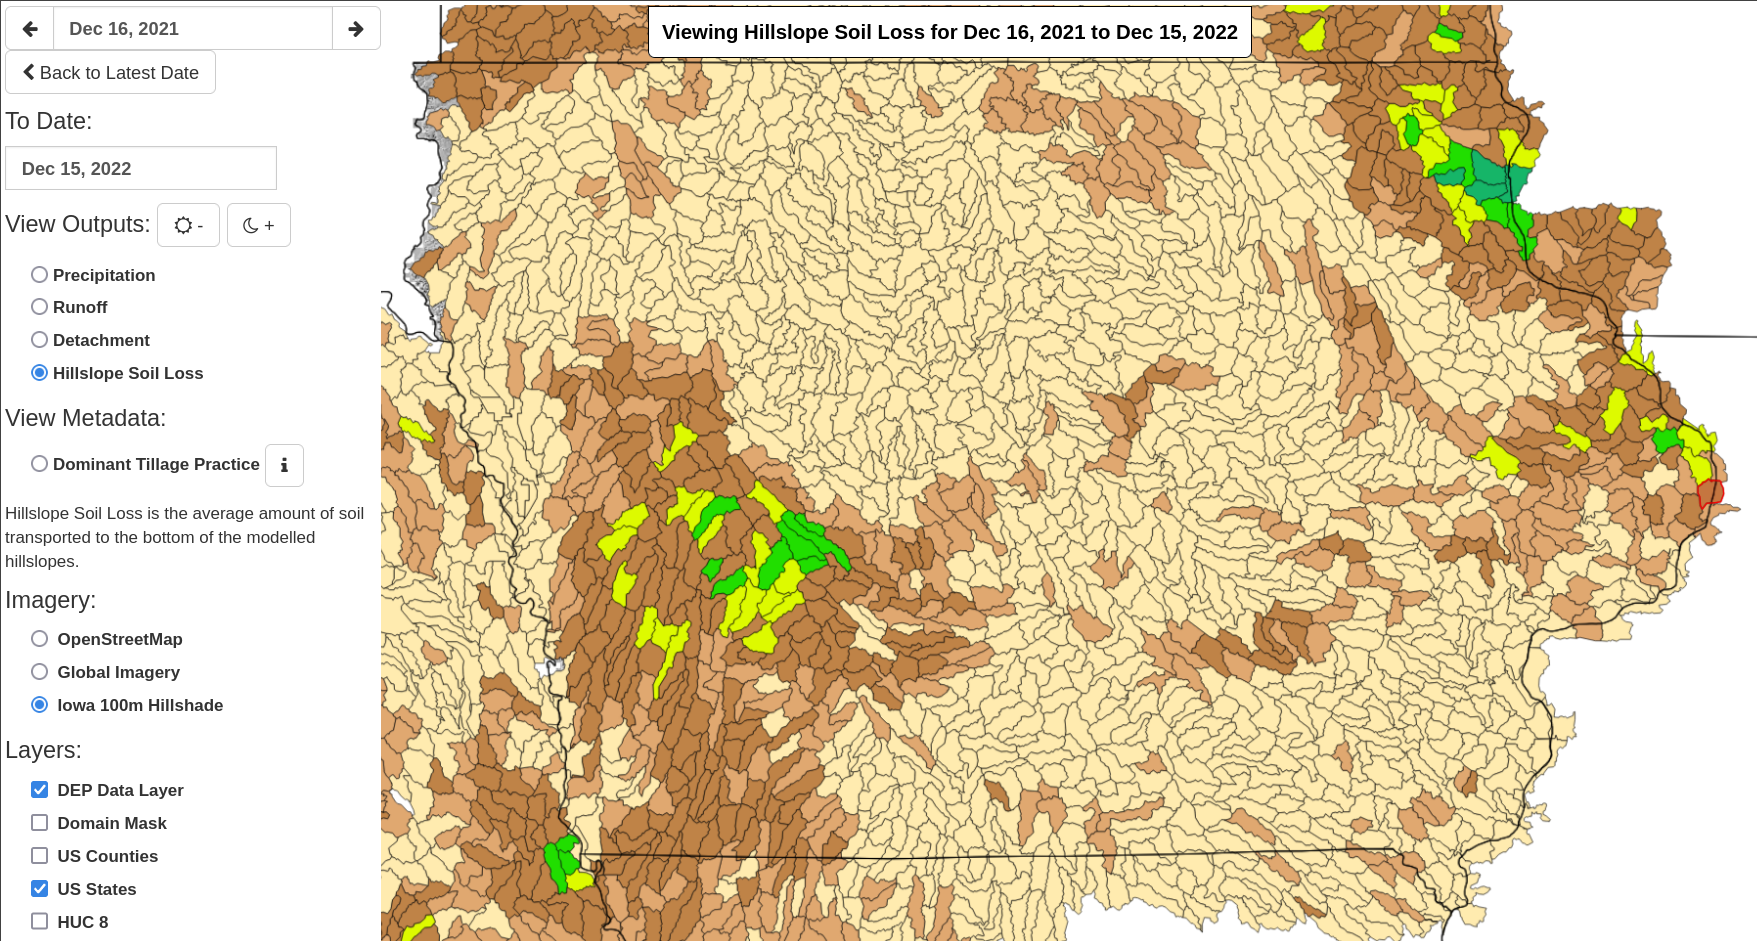
\includegraphics[height=17em]{inc/dep_soilloss_map_20221215_168.png}
      \caption*{%
        \href{https://bit.ly/3HZyaRl}{\resizebox{!}{1.5ex}{\beamergotobutton{www}}}
        Interactive map from dailyerosion.org (change to hillslope soil loss)}
  \end{figure}
\end{frame}

\begin{frame}
  \frametitle{Water Erosion Prediction Project}
  \framesubtitle{A functional input computer models}

  \begin{table}[]
    \footnotesize
    %\begin{tabular}{@{}lllll@{}}
    \begin{tabular}{p{15ex}p{25ex}p{15ex}p{20ex}p{20ex}}
%      \toprule
      \small Output
      & \begin{tabular}[c]{@{}l@{}}\small Input\\ $X(t): \mathcal{T} \to
	  \mathbb{R}$\end{tabular}
      & \begin{tabular}[c]{@{}l@{}}\small Index\\ $t \in \mathcal{T}$\end{tabular}
      & \begin{tabular}[c]{@{}l@{}}\small Index subspaces\\ $t \in
	  \mathcal{T}_u$\end{tabular}
      & \small Mechanism
      \\
      \midrule
      Soil erosion
      & Slope
      & Distance
      & Hillslope position
      & Water flow \vspace{1ex}
      \\
    \end{tabular}
  \end{table}

  \begin{figure}
    \centering
    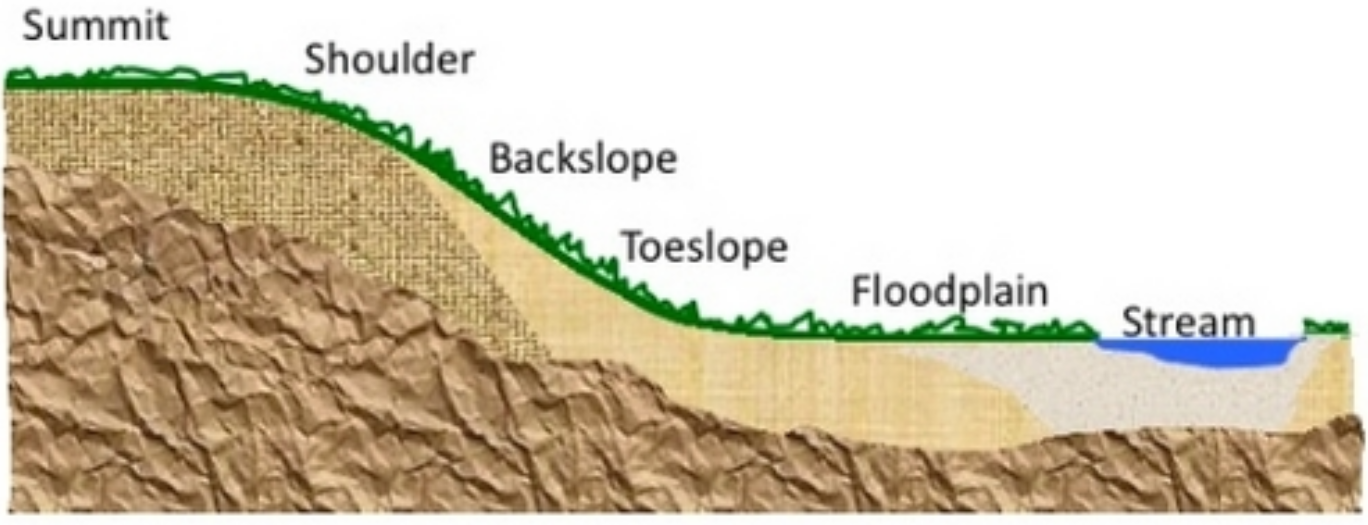
\includegraphics[height=10em]{inc/computer_model_hillslope_crop}
    \caption*{%
      \href{https://www.nature.com/scitable/knowledge/library/soil-carbon-storage-84223790/}{\resizebox{!}{1.5ex}{\beamergotobutton{www}}}
      Nature Education Knowledge}
  \end{figure}
\end{frame}

\begin{frame}
  \frametitle{Automatic Relevance Determination~\cite{neal1996,neal1998}}
  \framesubtitle{For a scalar input}

  $\mathrm{Cor}(y_i, y_j) = e^{-\theta {(x_i - x_j)}^2}$
  where $\theta\in\mathbb{R}^+$ is a weight driving the response correlation

  \begin{itemize}
  \item A predictor has little contribution on prediction as $\theta\to0^+$
    (flat)
  \item A predictor contributes to local predictions as $\theta\to\infty$
    (wiggly)
  \end{itemize}

  \begin{figure}
    \centering
    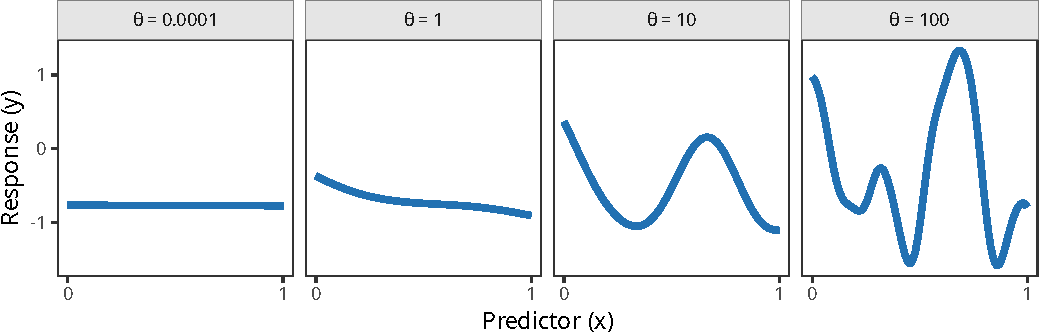
\includegraphics[height=10em]{inc/ard_response_profiles.pdf}
  \end{figure}

  \blankfootnote{
    $y\in\mathbb{R},x\in\mathbb{R}, i, j = 1, \dots, N, N\in\mathbb{N}$ \\
    \hspace{3.5ex}Fair warning: it's not so simple! relevance = input scale
    $\times$ linearity $\times$ predictive power~\cite{piironen2016}}
\end{frame}

\begin{frame}[c]
  \frametitle{\textsc{ARD} + Functional inputs}
  \framesubtitle{What is the state of the art?}

  %% A tikzdiagram goes here
  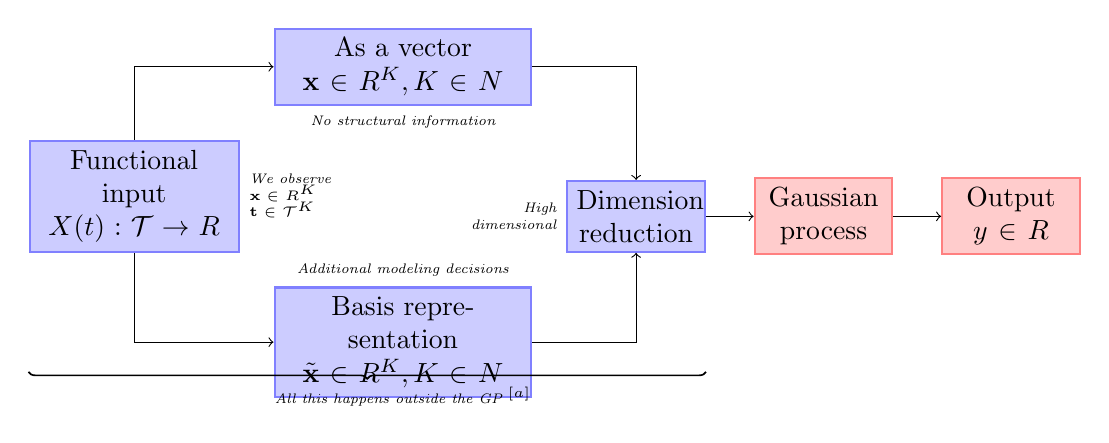
\begin{tikzpicture}
  [
  txtbox1/.style={rectangle,align=center,draw=blue!50,fill=blue!20,thick},
  txtbox2/.style={rectangle,align=center,draw=red!50,fill=red!20,thick},
  every label/.style={font=\itshape\tiny}
  ]

  \node (inp)  [txtbox1] at ( 0,  0) [text width=16ex]
  [label={[align=left]right:We observe \\ $\mathbf{x} \in \mathbb{R}^K$\\ $\mathbf{t}\in\mathcal{T}^K$}] {
    Functional input \\
    $X(t): \mathcal{T} \to \mathbb{R}$
  };
  \node (vec1) [txtbox1] [above right=4ex of inp]   [text width=20ex]
  [label=below:No structural information]{
    As a vector \\
    $\mathbf{x} \in \mathbb{R}^K, K \in \mathbb{N}$
  };
  \node (vec2) [txtbox1] [below right=4ex of inp]   [text width=20ex]
  [label=above:Additional modeling decisions]{
    Basis representation \\
    $\tilde{\mathbf{x}} \in \mathbb{R}^K, K \in \mathbb{N}$
  };

  \node (dred) [txtbox1] [above right=4ex of vec2] [text width=10ex]
  [label={[align=right]left:High\\dimensional}]
  {
    Dimension \\ reduction
  };

  \node (gp)   [txtbox2] [right=4ex of dred] [text width=10ex] {
    Gaussian \\ process
  };
  \node (out)  [txtbox2] [right=4ex of gp] [text width=10ex]  {
    Output \\ $y \in \mathbb{R}$
  };

  \node [below=6ex of vec2.north, label=below:All this happens outside the GP$~^{[a]}$] {
  };

  \draw [->] (inp.north) |- (vec1.west);
  \draw [->] (inp.south) |- (vec2.west);
  \draw [->] (vec1.east) -| (dred.north);
  \draw [->] (vec2.east) -| (dred.south);
  \draw [->] (dred.east) -- (gp.west);
  \draw [->] (gp.east)   -- (out.west);
  \path (inp.south west)
  edge[decorate,decoration={brace,mirror,raise=10ex},line width=.6pt]
  (inp.south west -| dred.south east);
\end{tikzpicture}

%%% Local Variables:
%%% mode: latex
%%% TeX-master: t
%%% End:


  \blankfootnote{
  % $~^{[1]}$\cite{muehlenstaedt2017,nanty2016,wang2017,tan2019,wang2019,betancourt2020,betancourt2020a,li2021} \,
  % $~^{[2]}$\cite{morris2012,kuttubekova2019}
%    $~^{[1]}$
  [a]
  Treat as vectors~\cite{iooss2009,nanty2016};
  reproject via splines~\cite{betancourt2020,betancourt2020a},
  functional principal component analysis~\cite{wang2017,wang2019},
  other basis representations~\cite{tan2019,li2021,striegel2022}\\
  \hspace{3.25ex}
  See also other attempts to incorporate the functional input structure into the
  GP~\cite{morris2012,muehlenstaedt2017,kuttubekova2019,Chen2021}
  \hyperlink{frm:litrev}{\resizebox{!}{1.5ex}{\beamergotobutton{appendix}}}
  }
\end{frame}

% Automatic Dynamic Relevance Determination ------------------------------------
\section{Automatic \textit{Dynamic} Relevance Determination \\
  {\tiny
    \href{https://doi.org/10.48550/arXiv.2209.00044}{arXiv:2209.00044}}
}

\begin{frame}
  \frametitle{Automatic Dynamic Relevance Determination}
  \framesubtitle{A framework for Gaussian Processes with functional inputs}

  \begin{align}
    y\in\mathcal{Y}
    &=\Reals \\
    X(t)\in\mathcal{X}
    &=\left\{X\colonfun\mathcal{T}\to\mathbb{R}, \int X(t)^2\mathrm{d}{t}<\infty\right\}
    \\
    t\in\mathcal{T}
    &=[0, 1]
      \only<2->{
      \\
    f
    &\hphantom{\colonfun\colonfun}
      \colonfun
      \hphantom{\colonfun\colonfun}\mathcal{X}\to\mathcal{Y} \\
    y_i
    &= f(X_i) \\
    f
    &\sim\mathcal{GP}(\cdot, \cdot)
      }
  \end{align}

  \blankfootnote{We assume that $t$ belongs in the unit interval w.l.o.g.}
\end{frame}

\begin{frame}
  \frametitle{Automatic Dynamic Relevance Determination}
  \framesubtitle{A framework for Gaussian Processes with functional inputs}

  \begin{align}
    \mathbf{y}
    &\sim \mathcal{N}\left(\mathbf{m}_f, \sigma_{f}^{2} \ \mathbf{R}_f
      + \sigma_{\varepsilon}^{2}\mathbf{I}\right) \\
    (\mathbf{m}_f)_i
    &= m_f(X_i) \\
    {\left(\mathbf{R}_f\right)}_{ij}
    &=
      \text{exp}\left\{
      -0.5 \phi^{-2} \ d_f(X_i, X_j)
      \right\}
      \only<2->{
    \\
    d_f(X_i, X_j)
    &= \int_{\mathcal{T}}
      \omega(t)
      {\left(X_i(t) - X_j(t) \right)}^2 dt
    \\
    \omega(t)
    &: \mathcal{T}\to\mathbb{R}^+
      }
  \end{align}

  \blankfootnote{
    $\sigma_{\varepsilon}^2 > 0$,
    $\sigma_{f}^2 > 0$,
    $\phi > 0$,
    $i, j = 1, \dots, N$,
    and $m_f(\cdot)$ is a mean function left unspecified for this presentation
  }
\end{frame}

% \begin{frame}
%   \frametitle{Automatic Dynamic Relevance Determination}
%   \framesubtitle{From ARD to ADRD}

%   %% tikz diagram
%   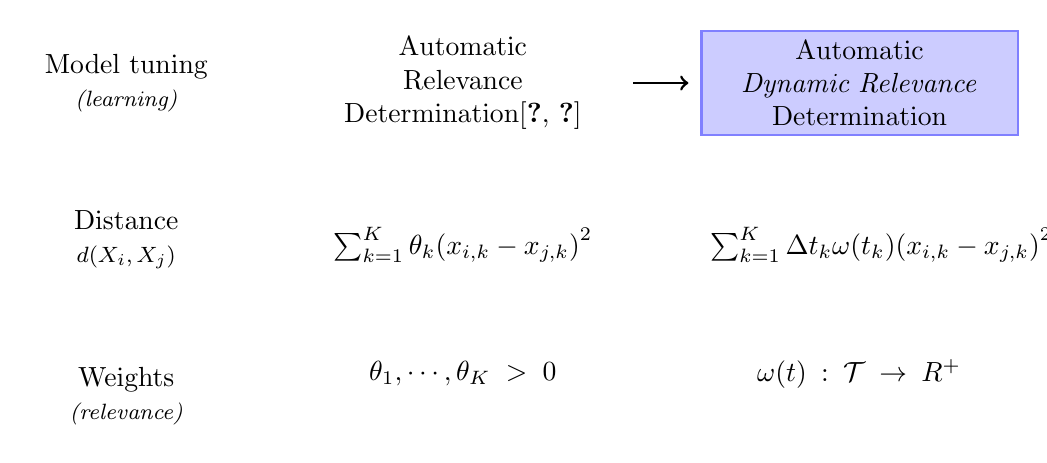
\begin{tikzpicture}
  [
  txtbox1/.style={rectangle,align=center,draw=blue!50,fill=blue!20,thick},
  every label/.style={font=\itshape\footnotesize}
  ]
  \tikzset{every node/.style={align=center}}
  \node (aspect1b)   at (0, 0)                        [text width=15ex] {
    Model tuning\\{\footnotesize \itshape (learning)}
  };
  \node (aspect2)    [below=of aspect1b]              [text width=15ex] {
    Distance\\{\footnotesize $d(X_i, X_j)$}
  };
  \node (aspect3)    [below=of aspect2]               [text width=15ex] {
    Weights\\{\footnotesize \itshape (relevance)}
  };
  %%%%%
  \node (solution1b) [right=of aspect1b]              [text width=25ex] {
    Automatic\\Relevance\\Determination\cite{neal1996,neal1998}
  };
  %%%%%
  \node (solution2b) [txtbox1] [right=of solution1b]  [text
  width=25ex]
  [visible on=<2->]{
    Automatic\\\textit{Dynamic Relevance}\\Determination
  };
  %%%%%
  \node (eq1b) [below=of solution1b] [text width=25ex] {
    % $\sum_{k=1}^K \frac{{(x_{i, k} - x_{j, k})}^2}{\ell_k^2}$
    $\sum_{k=1}^K \theta_k {(x_{i, k} - x_{j, k})}^2$
  };
  % \node (eq2b) [below=of solution2b] [text width=25ex]
  \node (eq2b) [right=of eq1b] [text width=25ex]
  [visible on=<2->]{
    % $\int_{\mathcal{T}}
    % \omega(t)
    % {\left(X_i(t) - X_j(t) \right)}^2 \mathrm{d}t$
    $\sum_{k=1}^K \Delta t_k \omega(t_k) {(x_{i, k} - x_{j, k})}^2$
  };
  %%%%%
  \node (par1b) [below=of eq1b] [text width=25ex]{
    % $\ell^{-2}_1, \cdots, \ell^{-2}_K > 0$
    $\theta_1, \cdots, \theta_K > 0$
  };
  % \node (par2b) [below=of eq2b] [text width=25ex]
  \node (par2b) [right=of par1b] [text width=25ex]
  [visible on=<2->]{
    $\omega(t): \mathcal{T} \to \mathbb{R}^+$
  };
  \draw[shorten >=1ex,shorten <=1ex,line width=1pt]
  [visible on=<2->] [->] (solution1b.east) -- (solution2b.west);
  % \draw[shorten >=1ex,shorten <=1ex,line width=1pt]
  % [visible on=<3->] [->] (eq1b.east) -- (eq2b.west);
  % \draw[shorten >=1ex,shorten <=1ex,line width=1pt]
  % [visible on=<4->] [->] (par1b.east) -- (par2b.west);
\end{tikzpicture}

%%% Local Variables:
%%% mode: latex
%%% TeX-master: t
%%% End:


%   \only<2->{
%     \blankfootnote{
%       \hyperlink{frm:riemann}{\resizebox{!}{1.5ex}{\beamergotobutton{appendix}}}
%       The Riemann approximation is used throughout this presentation
%     }
%   }
% \end{frame}

% \begin{frame}
%   \frametitle{Automatic Dynamic Relevance Determination}
%   \framesubtitle{A simple example}

%   We want to predict $y_j | y_i, X_i(t), X_j(t)$ via a zero-mean Gaussian
%   process for two observations $i, j$.

%   \begin{align}
%     \EV{y_j | y_i, X_i(t), X_j(t)}
%     &=
%     y_i e^{-\frac{1}{2}\phi^{-2} \int_\mathcal{T}
%     {\omega(t) \left(X_i(t) - X_j(t)\right)}^2\,\mathrm{d}t} \\
%     \VV{y_j | y_i, X_i(t), X_j(t)}
%     &=
%       \sigma_f^2
%       (1 - e^{-\phi^{-2} \int_\mathcal{T}
%     {\omega(t) \left(X_i(t) - X_j(t)\right)}^2\,\mathrm{d}t})
%   \end{align}

%   \begin{itemize}
%   \item A prediction is generated by comparing the two inputs profiles
%     everywhere, but \emph{especially} in higher weight index subspaces
%   \item Input differences in index subspaces with little weight
%     $\{t:\omega(t)\approx0\}$ will have limited to no impact on predictions
%   \end{itemize}
% \end{frame}

\begin{frame}
  \frametitle{Automatic Dynamic Relevance Determination}
  \framesubtitle{What do I need to use \textsc{ADRD} for my application?}

  \begin{itemize}
  \item Specify $\omega(t)$
    \begin{itemize}
    \item We introduced two parametric forms, a general form for basis
      expansion, and we explored three basis functions
    \item We discussed two relevance screening techniques
      \begin{itemize}
      \item Permutation-based screening \appendixlink{frm:pdfi}
      \item Riemann sum equivalence \appendixlink{frm:upscaled-weights}
      \end{itemize}
    \item We introduced two data analysis statistics
      \appendixlink{frm:statistics}
    \item Subject-matter expertise, prior knowledge about the problem
    \end{itemize}
  \item Evaluate integral from a finite representation
    \begin{itemize}
    \item Riemann sum as a general approximation
      \appendixlink{frm:integral-riemann}
    \item Closed-form expression for piecewise linear input and weights
      \appendixlink{frm:integral-pcws}
    \end{itemize}
  \item Estimate $\omega(t)$
    \begin{itemize}
    \item We discussed a set of weakly informative priors for
      the model parameters
      \appendixlink{frm:bayesian-priors}
    \item We carried out fully-Bayesian estimation framework via MCMC
      \appendixlink{frm:bayesian-estimation}
    \end{itemize}
  \end{itemize}
\end{frame}

\begin{frame}
  \frametitle{Automatic Dynamic Relevance Determination}
  \framesubtitle{Why do I want to use \textsc{ADRD} for my application?}

  \begingroup
  \setbeamersize{description width=-\labelsep}
  \begin{description}
  % \item[No dimension reduction] \mbox{}\\
  %   No need to lose information even for large $K$
  \item[Parsimony] \mbox{}\\
    $\omega(t)$ can be learned with fewer parameters than \textsc{ARD}
  \item[Smoothness] \mbox{}\\
    Smooth relevance function to penalize erratic or noisy \textsc{ARD} patterns
    \\
    e.g., $X(t_{k_1})$, $X(t_{k_2})$ and
    $X(t_{k_3})$ having disparate weights despite $t_{k_1} < t_{k_2} <
    t_{k_3}$ being close on the index space for the scale of the physical
    problem
  \item[Interpretability] \mbox{}\\
    $\omega(t) | \mathbf{y}$ may provide information about the underlying
    physical process
  \end{description}
  \endgroup
\end{frame}

\begin{frame}
  \frametitle{Automatic Dynamic Relevance Determination}
  \framesubtitle{Can I use \textsc{ADRD} along with $\dots$?}

  In principle, this framework is compatible with
  \begin{itemize}
  \item unregistered / unaligned observations
  \item correlation functions other than the exponential
  \item full and empirical Bayes, maximum likelihood, cross validation,
    other training paradigms
  \item big data approximations, e.g., local approximations
  \item distributed and GPU-accelerated computing
  \item smoothing models other than Gaussian Processes, e.g., KNN
  \end{itemize}
\end{frame}

% Weight function specification ------------------------------------------------
\section{Weight function specification %\\ {\small a case study} \\
  %{\tiny worked developed across several papers}
}

\begin{frame}
  \frametitle{Weight function specification}
  \framesubtitle{Asymmetric exponential weights}

  \begin{figure}
    \centering
    \includegraphics[height=10em]{inc/mls_weight_profiles}
  \end{figure}

  include t in the figure axis label, don't flip coordinates

  \begin{equation}
    \omega(t)
    =
    \text{exp}\left\{-(t - \tau)\lambda\kappa^s s\right\}
  \end{equation}

  \blankfootnote{
    Space:
    $\omega(t): \mathcal{T} = [0, 1] \to (0, 1]$,
    $s = \text{sign}(t - \tau)$,
    $\tau\in[0,1]$,
    $\lambda > 0$,
    $\kappa > 0$ \\
  }
\end{frame}

\begin{frame}
  \frametitle{Weight function specification}
  \framesubtitle{Basis expansion of the weights}

  \begin{equation}
    \log\omega(t)
    =
    \dots
  \end{equation}

  \blankfootnote{
    Space:
    $\omega(t): \mathcal{T} = [0, 1] \to (0, 1]$,
    $s = \text{sign}(t - \tau)$,
    $\tau\in[0,1]$,
    $\lambda > 0$,
    $\kappa > 0$ \\
    \hspace{3.25ex}
    Identifiability: (i) $\phi = 1$, (ii) $\psi_{c,0} = 0$,
    (iii) $\max_\mathcal{T}\omega(t) = 1$, or (iv)
    $\int_\mathcal{T}\omega(t)\dx{t} = 1$
  }
\end{frame}

\begin{frame}
  \frametitle{Weight function specification}
  \framesubtitle{Fourier expansion of the weights}

  \begin{figure}
    \centering
    \includegraphics[height=10em]{inc/few_weight_profiles}
  \end{figure}

  Show: bases on the left, weight functions on the right

  \begin{equation}
    \log\omega(t)
    \label{eq:few-log}
    =\psi_{c,0} + \sum_{g = 1}^{G} \psi_{c,g}\cos\left(2\pi gt\right)
      + \sum_{g = 1}^{G} \psi_{s,g}\sin\left(2\pi gt\right)
  \end{equation}

  \blankfootnote{
    Space:
    $\psi_{c,g},\psi_{s,g}\in\Reals$, $G\in\mathbb{N}$ \\
    \hspace{3.25ex}
    Identifiability: (i) $\phi = 1$, (ii) $\psi_{c,0} = 0$,
    (iii) $\max_\mathcal{T}\omega(t) = 1$, or (iv)
    $\int_\mathcal{T}\omega(t)\dx{t} = 1$
  }
\end{frame}

\begin{frame}
  \frametitle{Weight function specification}
  \framesubtitle{B-spline expansion of the weights}

  \begin{figure}
    \centering
    \includegraphics[height=10em]{inc/few_weight_profiles}
  \end{figure}

  Show: bases on the left, weight functions on the right

  \begin{equation}
    \log\omega(t)
    \label{eq:few-log}
    =\psi_{c,0} + \sum_{g = 1}^{G} \psi_{c,g}\cos\left(2\pi gt\right)
      + \sum_{g = 1}^{G} \psi_{s,g}\sin\left(2\pi gt\right)
  \end{equation}

  \blankfootnote{
    Space:
    $\psi_{c,g},\psi_{s,g}\in\Reals$, $G\in\mathbb{N}$ \\
    \hspace{3.25ex}
    Identifiability: (i) $\phi = 1$, (ii) $\psi_{c,0} = 0$,
    (iii) $\max_\mathcal{T}\omega(t) = 1$, or (iv)
    $\int_\mathcal{T}\omega(t)\dx{t} = 1$
  }
\end{frame}

\begin{frame}
  \frametitle{Weight function specification}
  \framesubtitle{Adaptive spline expansion of the weights}

  \begin{figure}
    \centering
    \includegraphics[height=10em]{inc/few_weight_profiles}
  \end{figure}

  Show: bases on the left, weight functions on the right

  \begin{equation}
    \log\omega(t)
    \label{eq:few-log}
    =\psi_{c,0} + \sum_{g = 1}^{G} \psi_{c,g}\cos\left(2\pi gt\right)
      + \sum_{g = 1}^{G} \psi_{s,g}\sin\left(2\pi gt\right)
  \end{equation}

  \blankfootnote{
    Space:
    $\psi_{c,g},\psi_{s,g}\in\Reals$, $G\in\mathbb{N}$ \\
    \hspace{3.25ex}
    Identifiability: (i) $\phi = 1$, (ii) $\psi_{c,0} = 0$,
    (iii) $\max_\mathcal{T}\omega(t) = 1$, or (iv)
    $\int_\mathcal{T}\omega(t)\dx{t} = 1$
  }
\end{frame}

\begin{frame}
  \frametitle{Weight function specification}
  \framesubtitle{Generative model}

  List with generative model
\end{frame}

\begin{frame}
  \frametitle{Weight function specification}
  \framesubtitle{Simulation study}

  Recovering the weight function from a well specified model
\end{frame}

% Daily Erosion Project --------------------------------------------------------
\section{Daily Erosion Project \\ {\small a case study} \\
{\tiny upcoming manuscript}}

\begin{frame}
  \frametitle{Data}
  \framesubtitle{How does landscape affect soil loss?}

  \begin{figure}
    \centering
    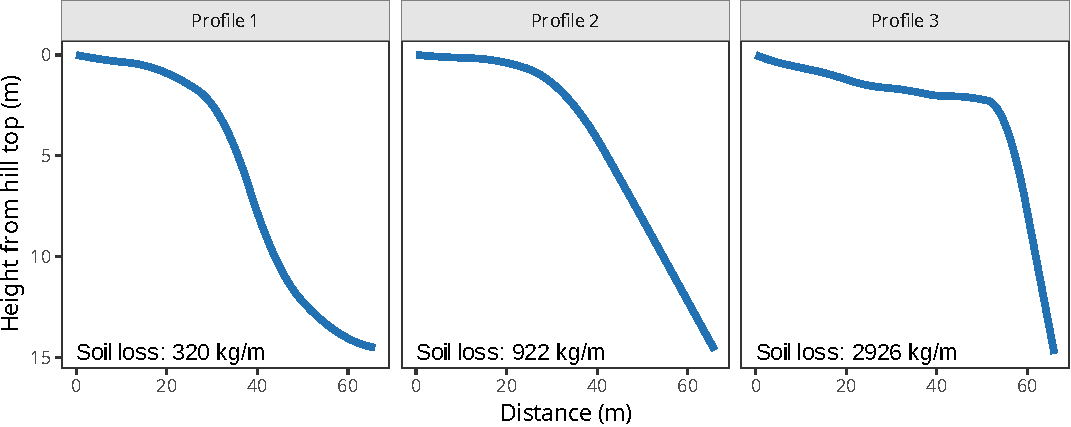
\includegraphics[height=12em]{inc/wepp_elevation_profiles}
    \caption*{
          \href{https://www.ars.usda.gov/midwest-area/west-lafayette-in/national-soil-erosion-research/docs/wepp/}{\resizebox{!}{1.5ex}{\beamergotobutton{www}}}
      Water Erosion Prediction Project version 2012.800
    }
  \end{figure}

  % {\tiny
  %   \href{https://www.ars.usda.gov/midwest-area/west-lafayette-in/national-soil-erosion-research/docs/wepp/}{\resizebox{!}{1.5ex}{\beamergotobutton{www}}}
  %     Water Erosion Prediction Project version 2012.800}
\end{frame}

\begin{frame}
  \frametitle{Data}
  \framesubtitle{Landscape characteristics and soil loss}

  \begin{itemize}
  \item Output: $y\in\mathbb{R}$ daily sediment delivery off-site (log kg/m)
  \item Inputs:
    \begin{itemize}
    \item Hillslope length: $x_1\in\mathbb{R}$ length (log m) of the overland flow
      element
    \item Mean slope: $x_2\in\mathbb{R}$ slope integral (log m/m) over the profile
    \item Slope profile: $X(t)\in\mathbb{R}$ slope steepness (log m/m) at $t$
    \item Normalized distance: $t\in[0, 1]$ from hilltop
    \item Discretization: $\{X(t_k) : t_k = k / 20, k = 1, \dots, 19\}$
    \item Climate, management, and soil parameters fixed constant
    \item Inputs are transformed to have approximately the same scale
    \end{itemize}
  \end{itemize}

  \vfill

  $\mathrm{Cor}(y_i, y_j) =
  \underbrace{\exp\{
    \int_\mathcal{T}
    \omega(t){(X_i(t) - X_j(t))}^2\,\mathrm{d}t\}
  }_{\mathrm{ADRD}}
  \times
  \underbrace{
    \vphantom{\int_\mathcal{T}}
      \exp\{\theta_1 {(x_{1i} - x_{1j})}^2\}
  \times
  \exp\{\theta_2 {(x_{2i} - x_{2j})}^2\}
  }_{\mathrm{ARD}}$
\end{frame}

\begin{frame}
  \frametitle{Methods}
  \framesubtitle{Implementation}

  \begin{itemize}
  \item 8 training and 8 test complementary sets with 1,000 runs each
  \item 6 plausible models
    \begin{itemize}
    \item Vector input with ARD
    \item Functional input with the following weight functions: (i) asymmetric
double exponential, (ii) asymmetric squared exponential, (iii) Fourier, (iv)
B-splines, (v) adaptive splines
    \end{itemize}
  \item
    \appendixlink{frm:bayesian-priors}
    Fully Bayesian estimation
    \begin{itemize}
    \item Hamiltonian Monte Carlo~\cite[ch. 5]{brooks2011}
    \item NUTS algorithm~\cite{hoffman2014} via
      Stan~\cite{standevelopmentteam2021}
    \item 1 long chain~\cite{raftery1992}
    \item Extensive search for an initial value
    \item 500 post-warmup iterations
    \item 1,500 posterior samples
    \end{itemize}
  \item \appendixlink{frm:validation}
    Multiple out-of-sample validation statistics
  \end{itemize}
\end{frame}

\begin{frame}
  \frametitle{Results}
  \framesubtitle{Model validation}

  \begin{figure}
    \centering
    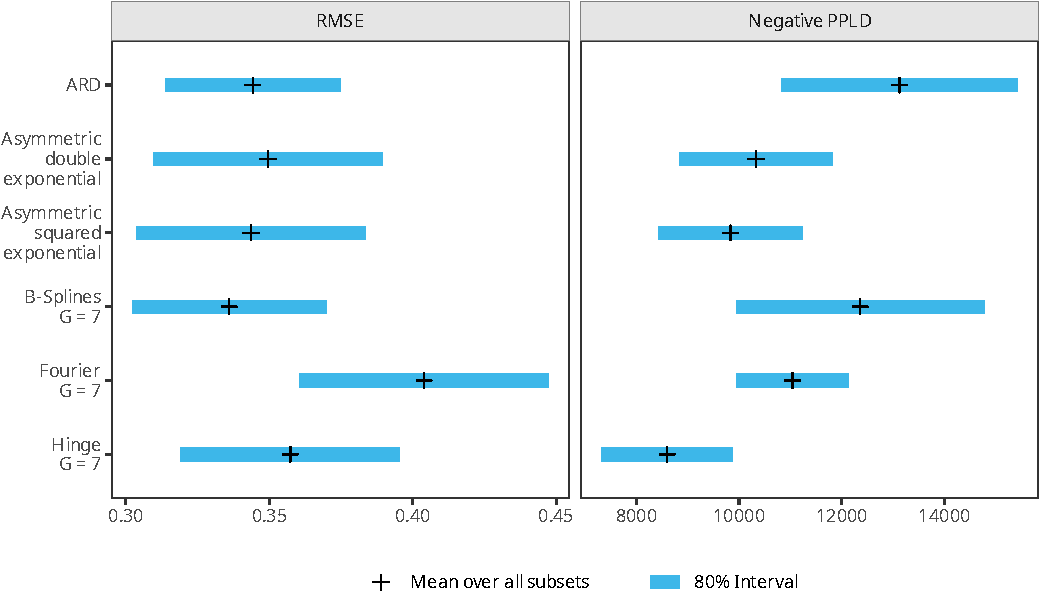
\includegraphics[height=15em]{inc/wepp_validation_summary_tiny_fsc140.pdf}
  \end{figure}

  \blankfootnote{
    $
    \hat{v}_1
    = {\tilde{M}}^{-1} \sum_{{\tilde{m}}=1}^{{\tilde{M}}} N^{-\frac{1}{2}}
    \norm{%
      \EV{\bm{y}_{*} | \bm{X}, \bm{X}_{*}, \bm{y}, {\bm{\theta}}_{{\tilde{m}}}}
      - \bm{y}_{*}}
    $ \\
    \hspace{3.25ex}
    $
    \hat{v}_2 = {\tilde{M}}^{-1} \sum_{{\tilde{m}}=1}^{{\tilde{M}}}
    p(\bm{y}_{*} | \bm{X}, \bm{X}_{*}, \bm{y},
    {\bm{\theta}}_{{\tilde{m}}})
    $
  }
\end{frame}

\begin{frame}
  \frametitle{Results}
  \framesubtitle{Posterior for model interpretation}

  \begin{figure}
    \centering
    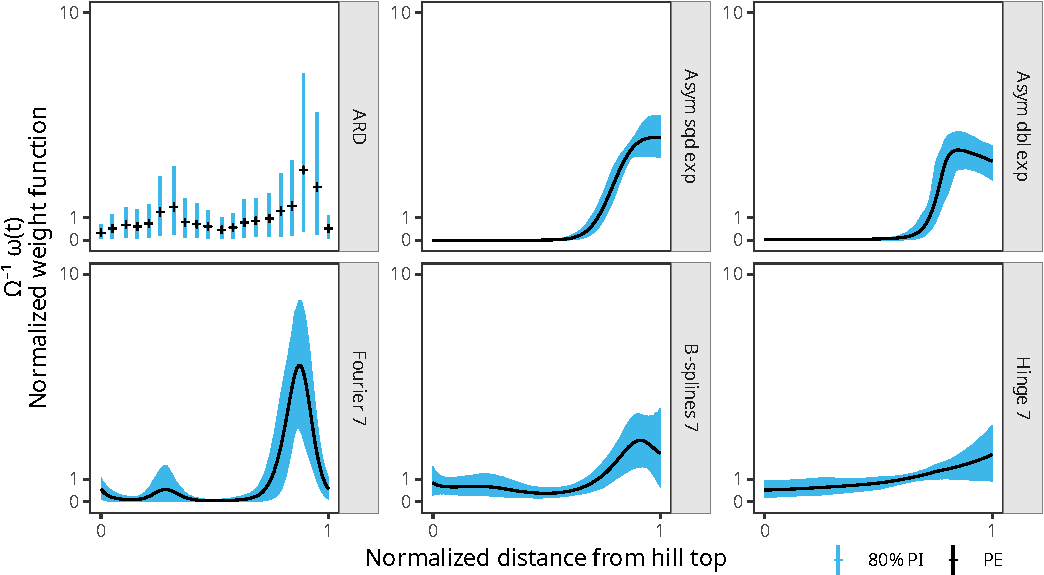
\includegraphics[height=15em]{inc/wepp_weight_posterior_tiny_fsc140.pdf}
  \end{figure}

  \blankfootnote{
    $
    p(\omega(t) | \bm{X}, \bm{y})
    \approx
    \{
    \omega_m(t) | \bm{X}, \bm{y}, \bm{\theta}_m
    : m = 1, \dots, M\}
    $
  }
\end{frame}

\begin{frame}
  \frametitle{Results}
  \framesubtitle{Posterior for model interpretation}

  \begin{figure}
    \centering
    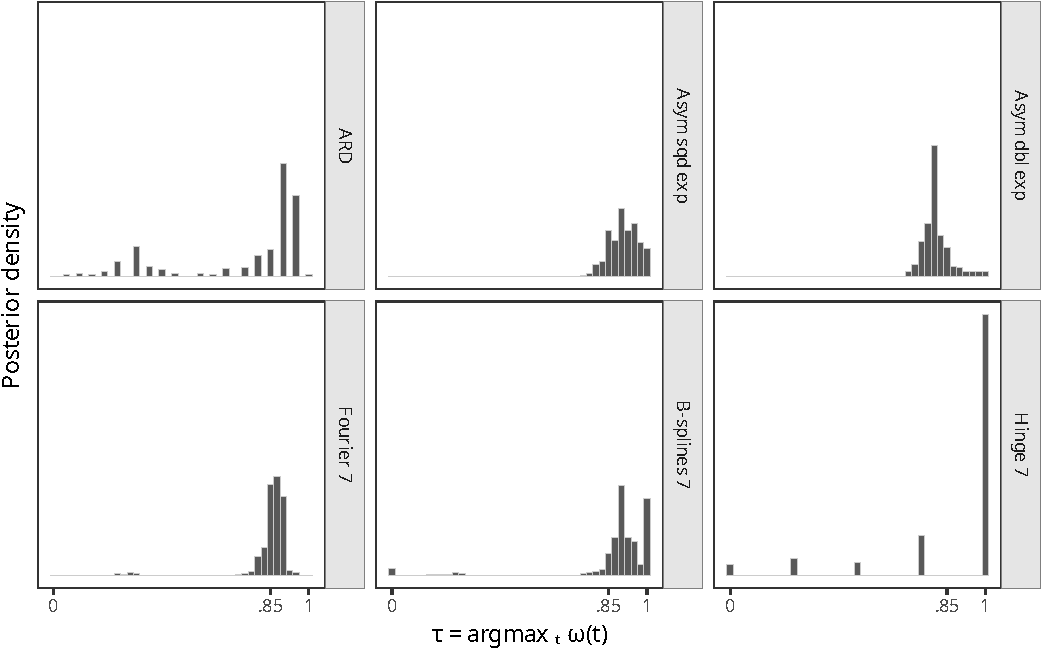
\includegraphics[height=15em]{inc/wepp_weight_argmax_tiny_fsc140.pdf}
  \end{figure}

  \blankfootnote{
    Most relevant location:
    $
    \tau = \argmax_{t\in\mathcal{T}}\omega(t)
    $,
    $
    p(\tau | \bm{X}, \bm{y})
    \approx
    \{
    \tau_m | \bm{X}, \bm{y}, \bm{\theta}_m
    : m = 1, \dots, M\}
    $
  }
\end{frame}

\begin{frame}
  \frametitle{Results}
  \framesubtitle{Posterior for model interpretation}

  \begin{figure}
    \centering
    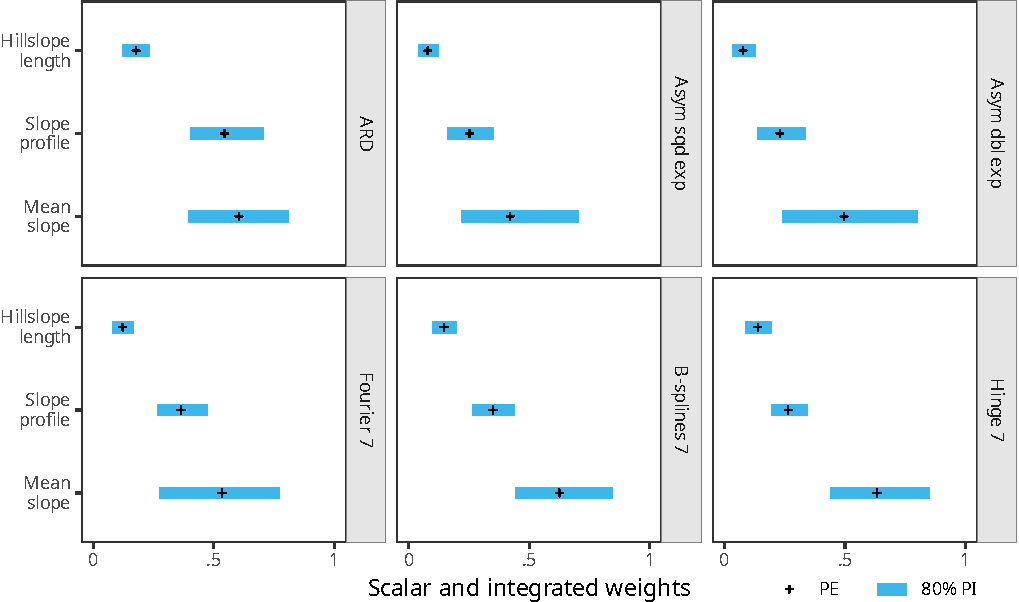
\includegraphics[height=15em]{inc/wepp_weight_integral_tiny_fsc140.pdf}
  \end{figure}

  \blankfootnote{
    Integrated weight:
    $
    \Omega = \int_\mathcal{T}\omega(t)\,\mathrm{d}t
    $,
    $
    p(\Omega | \bm{X}, \bm{y})
    \approx
    \{
    \Omega_m | \bm{X}, \bm{y}, \bm{\theta}_m
    : m = 1, \dots, M\}
    $
  }
\end{frame}

\begin{frame}
  \frametitle{Results}
  \framesubtitle{In summary}

  \begin{itemize}
  \item \textsc{ADRD} and \textsc{ARD} perform similarly prediction-wise
  \item \textsc{ADRD} and \textsc{ARD} agree on the overall relevance patterns
  \item Relevance seems to be very smooth in this computer model, as expected
  \end{itemize}
\end{frame}

% Discussion -------------------------------------------------------------------
\begin{frame}
  \frametitle{Discussion}
  \framesubtitle{Our contribution and open questions}

  Toward a framework for Gaussian processes with functional inputs
  $Y = f(X_1(u), X_2(v), \dots, x_1, x_2, \dots)$
  \begin{itemize}
    \footnotesize
  \item Framework for Gaussian processes with functional inputs
  \item Multiple scalar, vector, and functional inputs
  \item Flexible functional weight forms: \\
    parametric forms (ADE, ASE),
    basis expansions (Fourier, B-splines, adaptive splines)
  \item Closed-form expression for piecewise linear input and weights
  \item Case studies: Microwave Limb Sounder, Water Erosion Prediction Project
  \end{itemize}
  \vspace{3ex}

  Future work
  \begin{itemize}
    \footnotesize
  \item Functional of multiple indexes $Y = f(X(u, v))$
  \item Functional input with functional output $Y(u) = f(X(v))$
  \item Design of experiments:~An optimal design to learn $\omega(t)$?
    A design informed by $p(\omega(t) | \mathbf{X}, \mathbf{y})$
  \item Couple with local approximation (non-stationary, large matrix inversion)
  \end{itemize}
\end{frame}

% Closing slides ---------------------------------------------------------------
\begin{frame}[c]
  \frametitle{Acknowledgments}
  \centering

  {\small
    Benedict Neo, Jarad Niemi, Max D. Morris (ISU) \\
    Margaret Johnson, Joaquim Texeira, Microwave Limb Sounder team
    (JPL, Caltech) \\
    Rick Cruise, Brian Gelder, Daryl Herzmann (ISU) \\
    C-CHANGE:~Science for a Changing Agriculture \\
    Foundation for Food and Agriculture Research
  }

  \vfill

  {\huge Thank you!}

  \vfill

  {\tiny References and extra slides on the back}

  \href{ldamiano@iastate.edu}{\beamergotobutton{mail}
    ldamiano@iastate.edu}

  \href{https://luisdamiano.github.io}{\beamergotobutton{www}
    https://luisdamiano.github.io}

  \href{https://github.com/luisdamiano/isu23}{\beamergotobutton{repo}
    https://github.com/luisdamiano/isu23}
\end{frame}

\appendix
\setbeamertemplate{bibliography item}{\insertbiblabel}
\begin{frame}[allowframebreaks]{References}
  \tiny
  \bibliographystyle{unsrt}
  \bibliography{references}
\end{frame}

% Appendix ---------------------------------------------------------------------
\section{Appendix}

\begin{frame}%
  \label{frm:litrev}
  \frametitle{Literature review}

  Computer experiment with functional inputs $X(t):
  \mathcal{T}\to\mathbb{R}$ \\
  input quantities varying over a continuum typically modeled as function of
  some index

  \begin{itemize}
  \item Treat input as vectors~\cite{iooss2009}
  \item Transform input to vectors, e.g.,
    splines~\cite{betancourt2020,betancourt2020a}, principal component
    analysis~\cite{nanty2016}, functional principal component
    analysis~\cite{wang2017,wang2019}, among other basis
    functions~\cite{tan2019,li2021,striegel2022}
  \item A weight function for time-varying inputs and outputs~\cite{morris2012}
  \item A weight function for functional inputs with an $L^2$ norm approximated
    via splines~\cite{muehlenstaedt2017}
  \item A lengthscale function modeled via trigonometric basis
    functions~\cite{kuttubekova2019}
  \item A lengthscale for the functional input frequency~\cite{Chen2021}
  \end{itemize}

  \vfill{}
  Although functional input computer experiments are not uncommon,
  general methodology for functional input Gaussian processes is limited
\end{frame}

\begin{frame}%
  \label{frm:statistics}
  \frametitle{Automatic Dynamic Relevance Determination}
  \framesubtitle{Data analysis statistics}

  The weight function drives relevance over the index space by allowing the
  input profile square difference to contribute locally at varying degrees
  \begin{align}
    d_\omega(X_i, X_j)
    &= \phi^{-2}\int_{\mathcal{T}}
      \omega(t)
      {\left(X_i(t) - X_j(t) \right)}^2\dx{t}
  \end{align}

  \begin{itemize}
  \item The maximum relevance location statistic
    captures the point in the index space where the output responds most
    strongly and nonlinearly to changes in the functional input
    \begin{align}
      \label{eq:01-adrd-maximum-relevance-location}
      \tau&\coloneqq\argmax_{t\in\mathcal{T}}\omega(t),%\\
    \end{align}
  \item The scaled integrated weight statistic is a global measure that
    summarizes a functional input total relevance by integrating out the index
    variable
  \begin{align}
    \label{eq:01-adrd-scaled-integrated-weight}
    \Omega&\coloneqq\phi^{-2}\int_\mathcal{T}\omega(t)\dx{t},%\\
  \end{align}
  \end{itemize}
\end{frame}

\begin{frame}%
  \label{frm:integral-riemann}
  \frametitle{Integral evaluation with a finite representation}
  \framesubtitle{Riemann approximation}

  Consider a partition of the index interval $\left\{ t_k: t_0 = 0 \le t_1 <
    \cdots < t_K \le t_{K+1} = 1 \right\}$.
  %
  \begin{equation}
    \label{eq:01-adrd-integrand}
    d_{\omega}
    =\phi^{-2}\int_0^1 \w(t) \, {(X_i(t) - X_j(t))}^2 \dt
    =\phi^{-2}\sum_{k = 1}^{K + 1}
    \underbrace{
      \int_{t_{k-1}}^{t_k} \w(t) \, {(X_i(t) - X_j(t))}^2
      \dt}_{C_k}.
  \end{equation}
  %
  For the trapezoidal approximation, we set
  \begin{equation}
    C_k
    =\left(t_{k} - t_{k - 1}\right) \frac{
      \omega(t_{k}) {\left(x_{i, k} - x_{j, k}\right)}^2 +
      \omega(t_{k-1}) {\left(x_{i, {k-1}} - x_{j, {k-1}}\right)}^2
    }{2}.
  \end{equation}

  Since
  $S_k = e^{\phi^{-2} C_k}$ is positive semidefinite for fixed $k$, so
  is the product $S = \prod_{k} e^{\phi^{-2} C_k}$.
\end{frame}

\begin{frame}%
  \label{frm:integral-pcws}
  \frametitle{Integral evaluation with a finite representation}
  \framesubtitle{Closed-form expression for piecewise input and weight functions}

  Consider a partition of the index interval $\left\{ t_k: t_0 = 0 \le t_1 <
    \cdots < t_K \le t_{K+1} = 1 \right\}$.
  %
  \begin{equation}
    \label{eq:01-adrd-integrand}
    d_{\omega}
    =\phi^{-2}\int_0^1 \w(t) \, {(X_i(t) - X_j(t))}^2 \dt
    =\phi^{-2}\sum_{k = 1}^{K + 1}
    \underbrace{
      \int_{t_{k-1}}^{t_k} \w(t) \, {(X_i(t) - X_j(t))}^2
      \dt}_{C_k}.
  \end{equation}
  %
  Assume now that $\omega(t)$ and $X(t)$ are both piecewise linear over $[t_{k-1},
  t_{k}]$ so that $\omega(t) = \alpha_0 + \alpha_1 \, t$ and
  ${X_i(t) - X_j(t)} = \beta_0 + \beta_1 \, t$
  for some $\alpha_0, \alpha_1, \beta_0, \beta_1\in\mathbb{R}$.
  Then,
  \begin{equation}
    \label{eq:01-adrd-linweight-lininput}
    % from sympy import *
    % init_printing()
    % b0, b1, a0, a1, t, t0, t1 = symbols('b_0 b_1 a_0 a_1 t t_0 t_1')
    % integrate((a0 + a1 * t) * (b0 + b1 * t)**2, t)
    % integrate((a0 + a1 * t) * (b0 + b1 * t)**2, (t, t0, t1))
    \begin{split}
      C_k=\,
      &
      \alpha_0\beta_0^2
      \,\left({t_{k} - t_{k-1}}\right)
      +
      2^{-1}
      \left(
        2\alpha_0\beta_0\beta_1 + \alpha_1\beta_0^2
      \right)
      \,\left({t^2_{k} - t^2_{k-1}}\right)
      + \\
      &3^{-1}
      \left(\alpha_0\beta_1^2 + 2\alpha_1\beta_0\beta_1\right)
      \,\left({t^3_{k} - t^3_{k-1}}\right)
      +
      4^{-1}
      \alpha_1\beta_1^2
      \,\left({t^4_{k} - t^4_{k-1}}\right).
    \end{split}
  \end{equation}
\end{frame}

\begin{frame}%
  \label{frm:bayesian-priors}
  \frametitle{Fully Bayesian estimation}
  \framesubtitle{Parameter priors}

  We generally recommend the following independent weakly informative priors for
  cases where there is no domain-specific information about the relevance profile.
  \begin{itemize}
  \item Asymmetric exponential functions:
    $\tau \sim \textsc{Beta}(1, 1)$,
    $\lambda \sim \textsc{N}^{+}(0, 10)$,
    $\log(\kappa) \sim \textsc{N}(0, 1)$
  \item Fourier expansion of the weight:
    $\psi_g\sim\textsc{N}(0, g^{-2}\sigma^2_\psi)$ with
    $\sigma_\psi\sim\textsc{C}^+(0, 1)$, $\sigma_\psi\sim\textsc{N}^+(0, 1)$,
    or fixing $\sigma_\psi = 1$
  \item Basis expansion of the weight general form:
    $\psi_g \sim \textsc{N}(0, A)$ for some constant
    $A>0$ representative of the basis function scale, e.g., $A = 10$.
  \item Scale: $\phi \sim \textsc{InvGamma}(5, 5)$ to avoid
    values extremely close to zero or large, which may lead to numerical issues
    due to posterior density flattening
  \item Standard deviations: $\sigma_f, A^{\frac{1}{2}}\sigma_{\varepsilon}
    \iid \textsc{N}^{+}(0, 1)$ for some constant $A>0$
    representative of the signal-to-noise ratio, e.g., $A = 10$.
  \end{itemize}
\end{frame}

\begin{frame}%
  \label{frm:bayesian-estimation}
  \frametitle{Fully Bayesian estimation}
  \framesubtitle{Parameter estimation}

  \begin{itemize}
  \item We denote the parameter vector by $\bm{\theta} =
    (\bm{\theta}_{d}, \sigma_f^2, \sigma_{\varepsilon}^2)$, where
    $\bm{\theta}_{d}$ encompasses the unknowns for a specific choice of
    $d(X_i, X_j)$, e.g., $\bm{\theta}_{d} = (\phi, \lambda, \kappa, \tau)$.
  \item Let $\mathbf{X}$ be the training input matrix, $\mathbf{m}_y =
    m_y(\mathbf{X})$ the mean vector with %elements
    ${(\mathbf{m}_y)}_{i} = m_y(\mathbf{x}_i)$, and $\mathbf{S}_y =
    s_y(\mathbf{X})$ the covariance matrix with %elements
    ${(\mathbf{S}_y)}_{i, j} = s_y(X_i, X_j | {\bm{\theta}})$.
  \item Draw samples from the posterior $\bm{\theta}_m\sim\log p(\bm{\theta} |
    \mathbf{y}, \mathbf{X})$, $m = 1, \dots, M\in\mathbb{N}$
  \end{itemize}
  \begin{align}
    \label{eq:margina-likelihood}
    \log p(\mathbf{y} | \mathbf{X}, \bm{\theta})
    =& -\frac{1}{2}
       {(\mathbf{y} - \mathbf{m}_y)}^\top
       {\mathbf{S}_y}^{-1}
       {(\mathbf{y} - \mathbf{m}_y)}
       -\frac{1}{2}
       \log | \mathbf{S}_y |
       - \frac{n}{2} \log 2\pi \\
    \label{eq:parameter-posterior}
    \log p(\bm{\theta} | \mathbf{y}, \mathbf{X})
    \propto&
             \log p(\mathbf{y} | \mathbf{X}, \bm{\theta}) +
             \log p(\bm{\theta}).
  \end{align}

\end{frame}

\begin{frame}%
  \label{frm:validation}
  \frametitle{Validation statistics}

  \newcommand{\predmean}{\hat{\mathbf{m}}^{y}_*}
  \newcommand{\predvar}{\hat{\mathbf{S}}^{y}_*}
  \newcommand{\postpred}{\hat{p}^{y}_*}

  \begin{itemize}
  \item   Let
    $\hat{\mathbf{m}} = \predmean = \{\hat{m}_{*n}: n = 1, \dots, N\} =
    \EV{\mathbf{y}_* | \mathbf{y}, \mathbf{X}, \mathbf{X}_*}$
    and
    $\hat{\mathbf{S}} = \predvar = \VV{\mathbf{y}_* |
      \mathbf{y}, \mathbf{X}, \mathbf{X}_*}$
    be the predictive mean vector and covariance matrix.
  \item  Define the
    prediction error vector $\mathbf{e} = \mathbf{e}_{*}^{y} =
    \mathbf{y}_{*} - \hat{\mathbf{m}}$.
  \item Define the square Mahalanobis distance $D^2
    = \mathbf{e}^{\transp} \hat{\mathbf{S}}^{-1} \mathbf{e}$.
  \item   Let $\bar{y}_* = N^{-1} \sum_{n=1}^{N} y_{*n}$ be the test output
    mean.
  \end{itemize}

  \begin{center}
    \begin{tabular}{lrl}
      RMSE
      & $v_{\textsc{RMSE}}$ =
      & $N^{-\frac{1}{2}} \norm{\mathbf{e}}$ \\
      nPPLD
      & $v_{\textsc{nPPLD}}$ =
      & $
        \frac{1}{2} \log \lvert \hat{\mathbf{S}} \rvert
        +D^2
        +\frac{n}{2} \log 2 \pi
        $
      \\
      MAPE
      & $v_{\textsc{MAPE}}$ =
      & $N^{-1} \sum_{n = 1}^{N} |e_n / y_n|$ \\
      $R^2$
      & $v_{\textsc{R2}} $ =
      & $1 -%
        \norm{\mathbf{e}}^{2}
        \norm{\mathbf{y}_* - \bar{y}_*}^{-2}$ \\
      nCRPS
      & $v_{\textsc{nCRPS}}$ =
      & $
        \log \lvert \hat{\mathbf{S}} \rvert%
        +D^2
        $
    \end{tabular}
  \end{center}
\end{frame}

\begin{frame}%
  \label{frm:upscaled-weights}
  \frametitle{Dynamic relevance screening}
  \framesubtitle{Riemann sum equivalence}

  \begin{itemize}
  \item Recall the Riemann sum approximation to the integral
    \begin{align}
      \tilde{d}_{\textsc{ADRD}}(X_i, X_j)
      &\approx
        \phi^{-2}\sum_{k=1}^{K} \Delta t_k\,\omega(t_k) {(x_{i,k} - x_{j,k})}^2.
    \end{align}
  \item If the functional input is completely simplified to a $K-$dimensional
    vector input, we have
    \begin{align}
      \label{eq:01-adrd-ard-norm}
      d_{\textsc{ARD}}(X_i, X_j)
      &= \sum_{k = 1}^{K}{\sigma_{x_k}^{-2}(x_{i,k} - x_{j, k})}^2,
        \sigma_{x_k}^2 > 0.
    \end{align}
%    for $\sigma_{x_k}^2 > 0 \ \forall \ k = 1, \dots, K \in \mathbb{N}$.
  \item We set an equality and obtain
    \begin{align}
      \phi^{-2}\omega(t_k)
      &\approx {\Delta t_k}^{-1} \sigma^{-2}_{x_k}, k = 1,\dots, K
    \end{align}
  \item Visualize the upscaled scalar weights learned by an \textsc{ARD} model
  \end{itemize}
\end{frame}

\begin{frame}%
  \label{frm:pdfi}
  \frametitle{Dynamic relevance screening}
  \framesubtitle{Permutation Feature Dynamic Importance}

  \begin{itemize}
  \item We want to study the sensitivity of predictive accuracy to the
    information contained in different index subspaces
  \item We quantify the change in the validation statistics as we permute pieces
    of the input profile
  \item Let
    $\left\{\mathrm{T}_u\right\}_{u=1}^{U}, U \in \mathbb{N}$ form a
    partition of the index space $\mathcal{T}$.
  \item Let $\underline{\mathbf{x}}_{i,u} = [\mathbf{x}_{i,1}\cdots
    \mathbf{x}_{i',u}\cdots\mathbf{x}_{i,U}]$ be the corrupted input vector
    where $i' \ne i$ is chosen by random permutation, and
    $\underline{\mathbf{X}}_u$ the corrupted input matrix
  \item Train an $d_{\textsc{ARD}}(\cdot)$ model with $\theta_k > 0 \
    \forall \ k = 1, \dots K$ on $\mathbf{X}$
  \item Validate on
    $\underline{\mathbf{X}}_{*u}$ instead of $\mathbf{X}_{*}$
  \item Compare the validation statistic
    produced with the corrupted test input matrix to the
    reference point via the deterioration statistic $\Delta_{u} =
    \underline{v}_{u} - v$.
  \item The higher the increase in the loss statistic due to the permutation
    in the input block associated with the $u$-th index interval, the more
    reliant prediction accuracy is on the corresponding index
    subspace.
  \end{itemize}
\end{frame}

\end{document}
